\documentclass{exam}
\usepackage[utf8]{inputenc}
\usepackage{lmodern}
\usepackage{microtype}

% \usepackage[parfill]{parskip}
\usepackage[dvipsnames]{xcolor}
\usepackage{amsmath}
\usepackage{amsfonts}
\usepackage{amsthm}
\usepackage{siunitx}
\DeclareSIUnit\year{yr}
\DeclareSIUnit\foot{ft}
\DeclareSIUnit\litre{\liter}

\usepackage{skull}

\usepackage{pgfplots}
\usepgfplotslibrary{polar}
\pgfplotsset{compat=1.11}
\usepackage{graphicx}
\usepackage{sidecap}
\sidecaptionvpos{figure}{c}
\usepackage{float}
\usepackage{gensymb}
\usepackage{tkz-euclide}
\usetkzobj{all}
\usepackage{commath}
\usepackage{hyperref}
\usepackage{enumitem}
\usepackage{wasysym}
\usepackage{multicol}
\usepackage{mathtools}
\usepackage{tcolorbox}
\usepackage{tabularx}
\usepackage[version=4]{mhchem}
\usepackage{changepage}
\usepackage{listings}
\lstset{basicstyle=\ttfamily\linespread{0.8}\small}

\renewcommand*{\thefootnote}{\fnsymbol{footnote}}

\newtheorem*{thm}{Theorem}
\newtheorem*{iden}{Identity}
\newtheorem*{lemma}{Lemma}
\newtheorem{obs}{Observation}
\theoremstyle{definition}
\newtheorem*{defn}{Definition}
\newtheorem*{ex}{Example}
\newtheorem{con}{Construction}
\newtheorem*{alg}{Algorithm}

\newtheoremstyle{break}
  {\topsep}{\topsep}%
  {\itshape}{}%
  {\bfseries}{}%
  {\newline}{}%
\theoremstyle{break}
\newtheorem*{bthm}{Theorem}

% russian integral
\usepackage{scalerel}
\DeclareMathOperator*{\rint}{\scalerel*{\rotatebox{17}{$\!\int\!$}}{\int}}

% \DeclareMathOperator*{\rint}{\int}

\pgfplotsset{vasymptote/.style={
    before end axis/.append code={
        \draw[densely dashed] ({rel axis cs:0,0} -| {axis cs:#1,0})
        -- ({rel axis cs:0,1} -| {axis cs:#1,0});
    }
}}

% \pointsinrightmargin
\boxedpoints
\pointname{}

\newcommand{\questioA}{\question[\texttt{\textbf{\color{Cerulean} A}}]}
\newcommand{\questioM}{\question[\texttt{\textbf{\color{PineGreen} M}}]}
\newcommand{\questioE}{\question[\texttt{\textbf{\color{WildStrawberry} E}}]}
\newcommand{\questioS}{\question[\texttt{\textbf{\color{Goldenrod} S}}]}
\newcommand{\questioO}{\question[\texttt{\textbf{\color{BurntOrange} O}}]}

\newcommand{\parA}{\part[\texttt{\textbf{\color{Cerulean} A}}]}
\newcommand{\parM}{\part[\texttt{\textbf{\color{PineGreen} M}}]}
\newcommand{\parE}{\part[\texttt{\textbf{\color{WildStrawberry} E}}]}
\newcommand{\parS}{\part[\texttt{\textbf{\color{Goldenrod} S}}]}
\newcommand{\parO}{\part[\texttt{\textbf{\color{BurntOrange} O}}]}

\newcommand{\subparA}{\subpart[\texttt{\textbf{\color{Cerulean} A}}]}
\newcommand{\subparM}{\subpart[\texttt{\textbf{\color{PineGreen} M}}]}
\newcommand{\subparE}{\subpart[\texttt{\textbf{\color{WildStrawberry} E}}]}
\newcommand{\subparS}{\subpart[\texttt{\textbf{\color{Goldenrod} S}}]}
\newcommand{\subparO}{\subpart[\texttt{\textbf{\color{BurntOrange} O}}]}

\newcommand{\mainHeader}[2]{\section*{NCEA Level 2 Mathematics\\#1. #2}}
\newcommand{\mainHeaderHw}[2]{\section*{NCEA Level 2 Mathematics (Homework)\\#1. #2}}


\begin{document}

\mainHeader{5}{Quadratic Modelling}

A linear function is one of the form
\begin{displaymath}
  f(x) = mx + c;
\end{displaymath}
we have already seen that the graph of such a function is a straight line.

The natural next step is to consider quadratic functions: those of the form
\begin{displaymath}
  f(x) = ax^2 + bx + c.
\end{displaymath}
Last year, we saw that the graphs of quadratic functions are parabolae; so we can use quadratic equations to model situations
which are vaguely parabolic.

\begin{ex}\leavevmode
  \begin{center}
    \includegraphics[width=0.7\textwidth]{dimer}
  \end{center}
  The following table gives the instantaneous rates of reaction for the dimerization reaction above.
  \begin{center}
    \begin{tabular}{|c|c|c|}\hline
      \textbf{Time} (min) & \textbf{Concentration of reactant} (M) & \textbf{Instantaneous reaction rate} (M/min)\\\hline
      0 & 0.0054 &\\\hline
      10 & 0.0044 & \num{8.0e-5}\\\hline
      26 & 0.0034 & \num{5.0e-5}\\\hline
      44 & 0.0027 & \num{3.1e-5}\\\hline
      70 & 0.0020 & \num{1.8e-5}\\\hline
      120 & 0.0014 & \num{8.0e-6}\\\hline
    \end{tabular}
  \end{center}
  It is known that this reaction is second-order: that is, the reaction rate is modelled by a quadratic function of the
  reaction concentration. Let's call the reaction rate at a particular concentration $ R(C) $; so
  \begin{displaymath}
    R(C) = XC^2 + YC + Z.
  \end{displaymath}
  By using the values in the table above, we have that
  \begin{align*}
    \num{8.0e-5} &= X \cdot (0.0044)^2 + Y (0.0044) + Z\\
    \num{5.0e-5} &= X \cdot (0.0034)^2 + Y (0.0034) + Z\\
    \num{3.1e-5} &= X \cdot (0.0027)^2 + Y (0.0027) + Z.
  \end{align*}

  Using \texttt{matlab} to find $ X $, $ Y $, and $ Z $ we have
  \begin{verbatim}
    >> syms X Y Z;
    >> eqn1 = 8.0e-5 == X * (0.0044)^2 + Y * (0.0044) + Z;
    >> eqn2 = 5.0e-5 == X * (0.0034)^2 + Y * (0.0034) + Z;
    >> eqn3 = 3.1e-5 == X * (0.0027)^2 + Y * (0.0027) + Z;
    >> [A,B] = equationsToMatrix([eqn1,eqn2,eqn3],[X,Y,Z]);
    >> linsolve(A,B);

    ans =

                                      6148914691236521356/3658604241285734375
        364782697339246960843864593812277/21596587553915600330621553957928960
    -453142685283050860204790059017259/16872334026496562758298089029632000000
  \end{verbatim}
  So our model is
  \begin{displaymath}
    R(C) \approx 1.6807 C^2 + 0.01689 C - \num{2.686e-5}.
  \end{displaymath}
  Graphing our model (blue) next to the original data (red), we see that the match is reasonable.
  \begin{center}
  \fbox{\begin{tikzpicture}
    \begin{axis}[
      /pgf/number format/1000 sep={},
      axis lines = center,
      xlabel = $ C $,
      ylabel = $ R(C) $
    ]
      \addplot[domain = 0.001:0.005, color = blue, samples = 100] {1.6807*x^2 + 0.01689*x - 2.686e-5};
      \addplot[color = red, mark = square] coordinates{(0.0044,8e-5)(0.0034,5e-5)(0.0027,3.1e-5)(0.0020,1.8e-5)(0.0014,8e-6)};
    \end{axis}
  \end{tikzpicture}}
  \end{center}
  This is useful because it allows us to predict the reaction rate for concentrations that we have not measured; alternatively, we can predict the
  reactant concentration given the reaction rate (which can be easily measured).
\end{ex}

Some situations require us to find a minimum or a maximum value. Suppose, for example, that we are asked the following.

\begin{ex}
  Find the dimensions of a rectangle with perimeter \SI{1000}{\metre} such that the area is maximised.

  \textit{Solution.} Later this year, we will learn a systematic way to solve optimisation problems like this. However, using calculus here would be
  like using a machine gun to kill a fly (although for some reason it is the favoured method of economics students)!

  Let us call the two side lengths $ x $ and $ y $; so we have that $ 1000 = 2x + 2y $ (so $ 500 = x + y $), and we want to minimise $ A = xy $. Substituting,
  we have $ A = x(500 - x) = 500x - x^2 $. The maximum value will be the vertex of this parabola, so we need to put this formula into
  the form $ A = -(x - b)^2 + c $; if we expand this, then $ A = -x^2 + 2xb - b^2 + c $ and so we want $ 2b = 500 $ and $ c - b^2 = 0 $.
  From these, we see that $ b = 250 $ and $ c = (250)^2 $. Hence $ A = -(x - 250)^2 + (250)^2 $; the vertex is at $ x = 250 $, and so $ y = 250 $: the area
  will be maximised when the rectangle is a square.
\end{ex}

\clearpage
\subsection*{Questions}
You might want to use a calculator or a computer to help you with some of the calculations: for example, solving
systems of equations or quadratic equations.
\begin{questions}
  \question Give the equation of the following parabola:
    \begin{center}
    \fbox{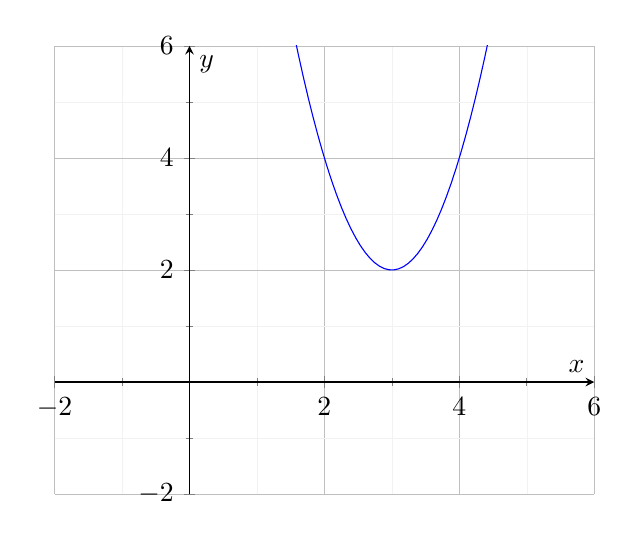
\begin{tikzpicture}
      \begin{axis}[
        axis lines = center,
        xlabel = $ x $,
        ylabel = $ y $,
        xmin = -2, xmax = 6,
        ymin = -2, ymax = 6,
        grid = both,
        grid style={line width=.1pt, draw=gray!10},
        major grid style={line width=.2pt,draw=gray!50},
        minor tick num=1
      ]
        \addplot[domain = -1:6, color = blue, samples = 100] {2*(x - 3)^2 + 2};
      \end{axis}
    \end{tikzpicture}}
    \end{center}
  \question
    \begin{parts}
      \part Find the vertices of the parabolae $ y = x^2 + 4x - 9 $ and $ y = -4x^2 + 2x - 1 $.
      \part More generally, show that the vertex of the parabola $ y = x^2 + bx + c $ is
            \begin{displaymath}
              \left(-\frac{b}{2}, c - \frac{b^2}{4}\right).
            \end{displaymath}
    \end{parts}
  \question
    \begin{parts}
      \part Find the equation of the parabola with vertex $ (2,3) $ that passes through $ (9,1) $.
      \part More generally, show that the equation of the parabola with vertex $ V(x_0, y_0) $ passing through $ A(x_1,y_1) $ is
            \begin{displaymath}
              y = \frac{y_1 - y_0}{(x_1 - x_0)^2}(x - x_0)^2 + y_0.
            \end{displaymath}
    \end{parts}
  \question One application of mathematical modelling is in chemical spectroscopy: it is possible to measure the absorbance
            of light by substances, which is proportional to the amount of the substance present.
            \begin{center}
              \begin{tabular}{|c|c|}\hline
                \textbf{Amount of protein} (\si{\micro\gram}) & \textbf{Absorbance}\\\hline
                0 & 0.099\\\hline
                5.0 & 0.185\\\hline
                10.0 & 0.282\\\hline
                15.0 & 0.345\\\hline
                20.0 & 0.425\\\hline
                25.0 & 0.483\\\hline
              \end{tabular}
            \end{center}
    \begin{parts}
      \part Use the values for 0, 5.0, and 25.0 micrograms to write down an equation for a parabolic model of this data.
      \part How accurately does this model predict the absorbance for 15 micrograms?
      \part A better model, taking into account all six data points, is found by computer to be
            \begin{displaymath}
              \text{amount of protein} = -0.000131429 A^2 + 0.0188686 A + 0.0982286.
            \end{displaymath}
            If the absorbance is measured experimentally to be 0.3, how much protein is present in the sample?
    \end{parts}
  \question Show that the $ x$-value of the vertex of a parabola is always halfway between the $ x$-intercepts.
\end{questions}

\end{document}
